\documentclass[10pt,mathserif]{beamer}
\setbeamertemplate{navigation symbols}{}
%\documentclass[handout]{beamer} % use this instead for handouts
\pdfoutput=1
%% Non beamer specific
\usepackage{amssymb}
\usepackage{wasysym}
\usepackage{epsfig,psfrag}
\usepackage{mathrsfs}
\usepackage{epigraph}
\usepackage{hyperref}
\usepackage{bm,amsmath}%  allow additional maths symbols
\usepackage{hyperref,url}     % for hyperreferences
\usepackage{graphicx}
\usepackage{subfigure}
\usepackage{framed}
\def\emptyline{\vspace{12pt}}
%% Beamer specifics

\graphicspath{{figs_pdf/}}

\usepackage{beamerthemeBoadilla}

\beamertemplateshadingbackground{white}{white}  % the 2 background colours
%\beamertemplatetransparentcovereddynamic  % covered items only grayed out

%\setbeamertemplate{headline}    % switch OFF headline 
%\setbeamertemplate{footline}    % switch OFF footline 
% RRK %%%%%%%%%%%%%%%%%%%%%%%%%%%%%%%%%%%%%%%%%%%%%%%%%%


\newcommand{\mathd}{\mathrm{d}}
\newcommand{\mathe}{\mathrm{e}}


\newcommand{\imag}{\mathrm{i}}

\newcommand{\vecuhat}{\widehat{\bm{u}}}
\newcommand{\vecnhat}{\widehat{\bm{n}}}
\newcommand{\hatu}{\widehat{u}}
\newcommand{\hatn}{\widehat{n}}
\newcommand{\vecx}{\bm{x}}

\newcommand{\vecv}{\bm{\mathrm{v}}}
\newcommand{\vecu}{\bm{\mathrm{u}}}

\newcommand{\myra}{\mathrm{Ra}}
\newcommand{\mypr}{\mathrm{Pr}}
\newcommand{\mynu}{\mathrm{Nu}}
\newcommand{\Tamb}{T_{\mathrm{amb}}}
\newcommand{\Thot}{T_{\mathrm{hot}}}
\newcommand{\Tcold}{T_{\mathrm{cold}}}


%\newcommand{\kappaf}{\kappa_{\mathrm{f}}}
%\newcommand{\nuf}{\nu_{\mathrm{f}}}

\newcommand{\kappaf}{\kappa_2}
\newcommand{\nuf}{\nu_2}
\newcommand{\kf}{k_2}
\newcommand{\alphaf}{\alpha_2}
\newcommand{\mypraf}{\mathrm{Pr}_2}

%\newcommand{\kappaa}{\kappa_{\mathrm{a}}}
%\newcommand{\nua}{\nu_{\mathrm{a}}}

\newcommand{\kappaa}{\kappa_3}
\newcommand{\nua}{\nu_3}
\newcommand{\ka}{k_3}
\newcommand{\alphaa}{\alpha_3}
\newcommand{\mypra}{\mathrm{Pr}_3}

\newcommand{\Je}{J_E}

\newcommand{\emphlon}[1]{\textcolor{blue}{\textbf{#1}}}

\definecolor{mygray}{HTML}{F8F8F9}

%\epigraphfontsize{\small\itshape}
%\setlength\epigraphwidth{8cm}
%\setlength\epigraphrule{0pt}


\begin{document}

%\input ../macros.tex

%%%%%%%%%%%%%%%%%%%%%%%%%%%%%%%%%%%%%%%%%%%%%%%%%%%%%%%%%%%%%%%%%%%%%%%%%%%

%%%% Setup Title Page %%%%%%%%%%%%%%%%%%%%%%%%%%%%%%%%%%%%%%%%%%%%%%%%%%%%%
\title[ACM40910:Modelling orientation dynamics using SDE]{Modelling the orientation dynamics of ``chaotic mixing``/ turbulence.}
\author[]{
Ian Towey \\
04128591
}
\date{\today}

\institute[]{
Msc Data and Computational Science\\
}
%%%%%%%%%%%%%%%%%%%%%%%%%%%%%%%%%%%%%%%%%%%%%%%%%%%%%%%%%%%%%%%%%%%%%%%%%%%

\begin{frame}
    \titlepage
\end{frame}

\section{Introduction}
\begin{frame}{Introduction : Why study turbulence}
\begin{columns}[t]						% the [t] option aligns the column's content at the top
\begin{column}{0.60\linewidth}

\begin{itemize}
\visible<2->{
\item It is a common phenomenon encountered in science and engineering.
}
\visible<3->{
\item No analytical theory to predict the evolution of turbulent flows, closure problem.
}    %	
\visible<4->{
\item Large scale direct numerical simulations of turbulence are computationally intractable.%would require a grid  with number of nodes proportional to $Re^{9/4}$
}    %	
\end{itemize}
\visible<5->{
\epigraph{``Turbulence is the most important unsolved problem of classical physics.``}{- \textup{Richard P. Feynman} \\ In The Feynman Lectures on Physics (1964). }
}    %	
\end{column}
  
\begin{column}{0.40\linewidth}
\begin{figure}
\begin{center}
\includegraphics[width=0.9\linewidth]{/home/ian/Desktop/eddy-davinci.jpg}
\end{center}
\begin{center}
\includegraphics[width=0.9\linewidth]{/home/ian/Desktop/jupiter.jpg}
\end{center}
\end{figure}
\end{column}
\end{columns}
\end{frame}

\section{Context}

\begin{frame}{Context of work}

\begin{columns}[t]						% the [t] option aligns the column's content at the top
\begin{column}{0.64\linewidth}
\visible<1->{Modelling orentation angle and growth rate of a tracer gradient in two-dimensional turbulence:
\begin{itemize}
\visible<2->{
\item Define 2-d turbulence model.
}
\visible<3->{
\item Define Orientation dynamics model.
}
\visible<4->{
\item Define the model of the orentation dynamics using a system of SDEs. Derive the corresponding Fokker-Planck PDE
}
\visible<5->{
\item Numerical Simulation of two-dimensional turbulence.
}
\visible<6->{
\item Solve Fokker-Planck numerically to find the PDF of the orientation angle and growth rate.
}
\visible<7->{
\item Compare the PDF of the orientation angle from the vorticity simulation vs and FP model.
}
\visible<8->{
\item Use uncertainty quantification methods to fit angle and growth rate PDF parameters to the simulated data.
}
\end{itemize}
}
\end{column}
\end{columns}
\end{frame}

\section{Theoritical Background}

\begin{frame}{Advection-Diffusion equation}
\begin{columns}[t]						% the [t] option aligns the column's content at the top
\begin{column}{0.64\linewidth}
\visible<1->{
\[
  \frac{\partial \theta}{\partial t} + \mathbf{u} \cdot \nabla \theta = \kappa \nabla^{2} \theta 
\]
}
\visible<2->{
\begin{itemize}
 \item $\mathbf{u}(x,t)$ is the velocity field
 \item $\theta$ is the concentration of some passive scalar (tracer)	
 \item $\kappa$ is the diffusion coefficient (in this context $\kappa = 0$)
 \item $\nabla \cdot \mathbf{u} = 0$ (incompressable flow)
\end{itemize}  
}
\visible<3->{
\vspace{10mm}
The model for the orientation dynamics will be dervied from the Advection-Diffusion equation
}
\end{column}
\end{columns}
\end{frame}

\begin{frame}{Vorticity Equation}
\begin{columns}[t]						% the [t] option aligns the column's content at the top
\begin{column}{0.64\linewidth}
\visible<1->{
\[
\frac{\partial \omega}{\partial t} + \mathbf{u} \cdot \nabla \omega = (-1)^p \nu_p \nabla^{2p} \omega + \nabla \times \mathbf{F} - \nabla \times \mathbf{D} 
\]
}
\visible<2->{
\begin{itemize}
 \item $\omega$ is the vorticity, describes the rotation of a fluid particle some point
 \item $\mathbf{u}(x,t)$ is the velocity
 \item $\nu$ is the viscosity
 \item $\mathbf{F}$ is a forcing term	
 \item $\mathbf{D}$ is a damping term	
\end{itemize}  
}
\end{column}
\end{columns}
\end{frame}

\begin{frame}{Orientation Dynamics}
\begin{columns}[t]						% the [t] option aligns the column's content at the top
\begin{column}{0.64\linewidth}
\visible<2->{
\[
  \frac{\partial \mathcal{B}}{\partial t} + \mathbf{u} \cdot \nabla \mathcal{B} = \mathcal{B} \cdot \nabla \mathbf{u}
\]
\[
  \mathcal{B} = (-\theta_{y},\theta_{x})
\]
}
\visible<3->{
\[
  \frac{d}{dt}\mathcal{|B|}^2 = - 2\mu \sin \zeta \mathcal{|B|}^2
\]
}
\visible<4->{
\noindent\rule{8cm}{0.4pt}
The growth rate of the tracer gradient is defined as
\begin{framed}
\emphlon{
\[
\Lambda = - 2\mu \sin \zeta
\]
}
\end{framed}
\visible<3->{
\begin{itemize}
 \item $\mu$ is the strain rate
 \item $\zeta$ orientation angle
\end{itemize}  
}
}
\end{column}
\end{columns}
\end{frame}


\begin{frame}{Stochastic Model  Equation Model}
\begin{columns}[t]						% the [t] option aligns the column's content at the top
\begin{column}{0.64\linewidth}
\visible<2->{
\begin{align*}
\gamma \frac{dX}{dt} &= w + ( -cos(X) +k\sqrt{\delta})Y +Z \\
\frac{dY}{dt} &= -\frac{Y}{\tau} + \frac{\sqrt{D_{Y}}}{\tau}\xi_{Y}  \\ 
\frac{dZ}{dt} &= -\frac{Z}{\tau} + \frac{\sqrt{D_{Z}(1-k^{2})}}{\tau}\xi_{Z} \\ 
\end{align*} 
}
\visible<3->{
Corresponding Fokker-Planck equation 
\[
\frac{\partial P}{\partial t} = \mathcal{L}_{OU}P - \frac{\partial}{\partial t}(VP)
\]
where 
\begin{tiny}
\begin{align*}
\mathcal{L}_{OU}P &= \frac{1}{\tau_{Y}}\frac{\partial}{\partial t}(y \circ) + \frac{1}{\tau^{2}_{Y}}\frac{\partial^{2}}{\partial y^{2}} + \frac{1}{\tau_{Z}}\frac{\partial}{\partial Z}(z \circ) + \frac{\rho}{\tau^{2}_{Z}}\frac{\partial^{2}}{\partial z^{2}} + \frac{2c\sqrt{\rho}}{\tau_{Y}\tau_{Z}}\frac{\partial^{2}}{\partial y \partial z} \\
\vspace{10mm}
V &= 2(w + y \cos x + z)
\end{align*}
\end{tiny}
}
\end{column}
\end{columns}
\end{frame}


\section{Numerical Simulation}
\begin{frame}{Numerical Simulation : Vorticity Equation}

\begin{columns}[t]						% the [t] option aligns the column's content at the top
\begin{column}{0.60\linewidth}
\begin{itemize}
\visible<2->{
  \item Periodic Boundary Conditions}
\visible<3->{
  \item Discretise the Vorticity equation}
\visible<4->{
  \item Convert discretised vorticity equation to fourier space}
\visible<5->{
  \item Save snapshots of $\omega$ at regular intervals}
\visible<6->{
  \item Extract emperical PDF of angle X statistically stable dataset}
\end{itemize}

\end{column}

\begin{column}{0.40\linewidth}
\begin{figure}
\begin{center}
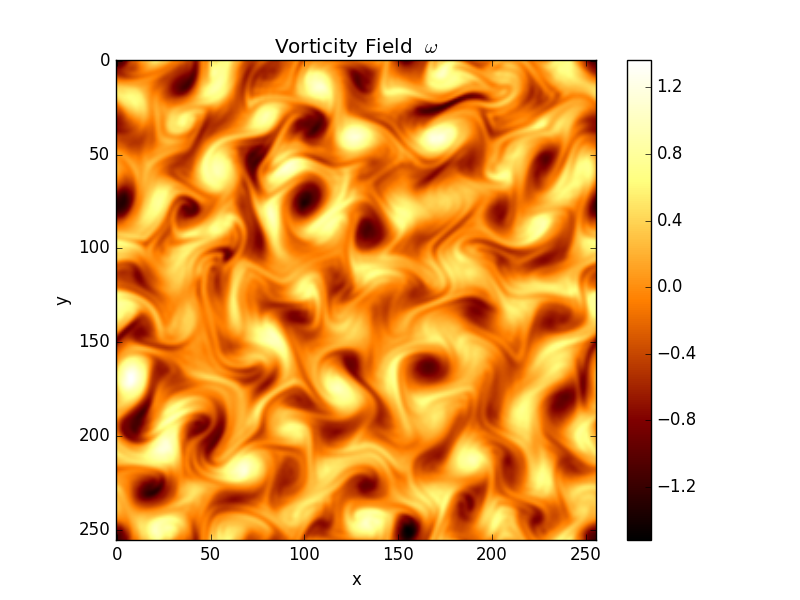
\includegraphics[width=0.9\linewidth]{/home/ian/Desktop/vorticity-field.png}
\end{center}
\end{figure}
\begin{figure}
\begin{center}
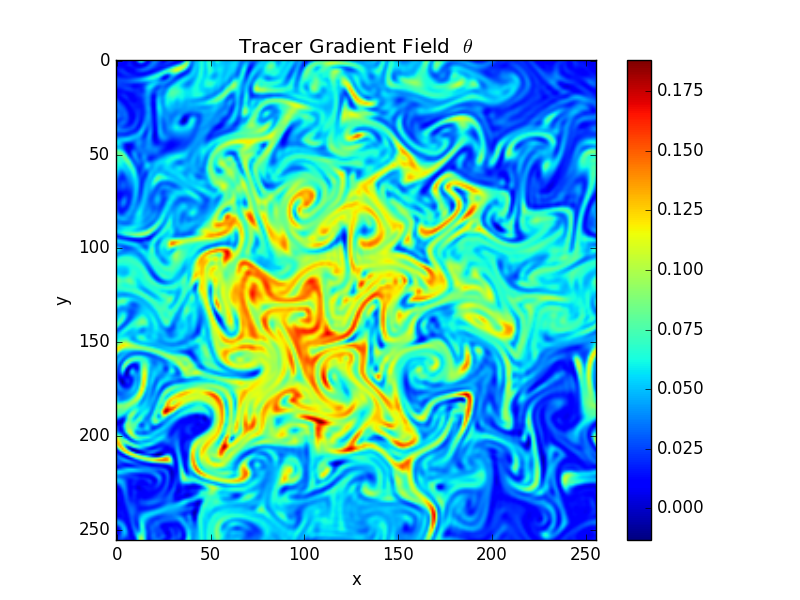
\includegraphics[width=0.9\linewidth]{/home/ian/Desktop/tracer-field.png}
\end{center}
\end{figure}
\end{column}
\end{columns}
\end{frame}

\begin{frame}{Numerical Simulation : Fokker Planck}

\begin{columns}[t]						% the [t] option aligns the column's content at the top
\begin{column}{0.60\linewidth}
\begin{itemize}
\visible<2->{
  \item Periodic Boundary Conditions}
\visible<3->{
  \item Solve for PDF of the Fokker-Plank}
\visible<4->{
  \item Extract marginal probability of X for the PDF of the angle X}
\visible<5->{
  \item Compute the PDF of the growth rate $\Lambda$ using the joint PDF of XY}
\end{itemize}
\end{column}
\end{columns}
\end{frame}


\section{Analysis of Results to date}

\begin{frame}{Analysis to date}
\begin{columns}[t]						% the [t] option aligns the column's content at the top
\begin{column}{0.60\linewidth}
\begin{itemize}
\visible<1->{
  \item Verify simulation of vorticity has reached a steady state}
\visible<2->{
  \item Compare the PDF of the angle X from the SIM vs the SDE model}
\visible<3->{
  \item Compare the PDF of the growth rate from th SIM vs the SDE model}
\end{itemize}

\end{column}
\begin{column}{0.40\linewidth}
\begin{figure}
\begin{center}
\includegraphics[width=0.9\linewidth]{/home/ian/Desktop/omega_variance.png}
\end{center}
\end{figure}
\end{column}
\end{columns}
\end{frame}


\section{Outstanding Work}
\begin{frame}{Outstanding Work}
\begin{itemize}
\visible<2->{
  \item Apply uncertainty quantification methods to the SDE/Fokker-Planck equation to fit the model parameters 
  }
\end{itemize}

\end{frame}

\section{Conclusions}
\begin{frame}{Conclusions}
\end{frame}

\section{Finished}
\begin{frame}{The End}
\end{frame}


\end{document}



